\chapter{Data Manipulation}

\section{Manipulating Geometrical Data}
\index{Manipulating geometrical data}

There is a small number of function to manipulate geometric data in \ogs. The common approach to the manipulation of \ogs input data is that it should be changed in a GIS or other specialised software of the user's choice which usually offers much more functionality for these things than \ogs ever could.

However, it is possible to set or change names for any geometrical object by right-clicking on the object and selecting \cmd{Set name...}\index{Setting names}\index{Changing names}. Upon saving the data again, the new or modified names will be saved in the corresponding file.

\subsubsection{Removing Duplicate Points}
\index{Removing geometric points}

Upon loading geometric data, the programme will check if any two geometric points are identical or \emph{almost} identical (within a small $\varepsilon$-range) and remove these points. GIS software often produces feature files that contain duplicate points which is not a problem within GIS but leads to all kinds of problems during tessellation of polygons or volumes as well as during a subsequent FEM simulation.

While the software will remove these duplicate points everytime a specific data set is loaded, it makes sense to save the cleaned data set and thus save loading time later on and be sure to work with a more suitable data set.

\bigskip

All other functions for manipulating geometry are associated with polylines and can be applied by right-clicking the ``Polylines'' item of any geometry in the Data View and then selecting \cmd{Connect Polylines...}.

\subsubsection{Connecting Polylines}
\index{Connecting polylines}
This function connects all the selected polylines to a single new polyline provided that the start- and end points of all segments are within the given maximum distance. The default maximum distance is $0.0$, meaning that start- and end points have to be identical. A name may be added to the resulting new polyline.

Note that if more than two start/end points are located within the given maximum distance, still only two of those points are connected. These points are chosen randomly. It is not advised to use a maximum distance that may lead to ambiguous results.

The newly created polyline is added to the geometry. All the polylines that are parts of this new line are still kept within the geometry.

\subsubsection{Creating Polygons by Closing Polylines}
\index{Creating polygons from polylines}
This function closes a (connected) polyline. Simply check `Close connected Polyline'. Again, if a name has been entered, this name will be assigned to the closed polyline.

\subsubsection{Creating Surfaces by Triangulating Polygons}
\index{Creating surfaces from polygons}
This function additionally creates a new surface by triangulating the newly created polygon. This simply requires checking `Create Surface from Polyline'. The newly created polyline has to be closed for that function to work. If a name has been entered, this name will be assigned to the surface.

\subsubsection{Merging geometries}
\index{Merging geometries}

Multiple geometry data sets can be merged to a single geometry by selecting \cmd{Tools\ra Mesh Generation...} from the menu. This will open a dialog showing all currently loaded geometries with the option select those data sets that should be merged. It is also possible to assign a name to the merged geometry.

\begin{figure}[tb]
  \centering
  \subfloat[Mapping based on DEM]{\frame{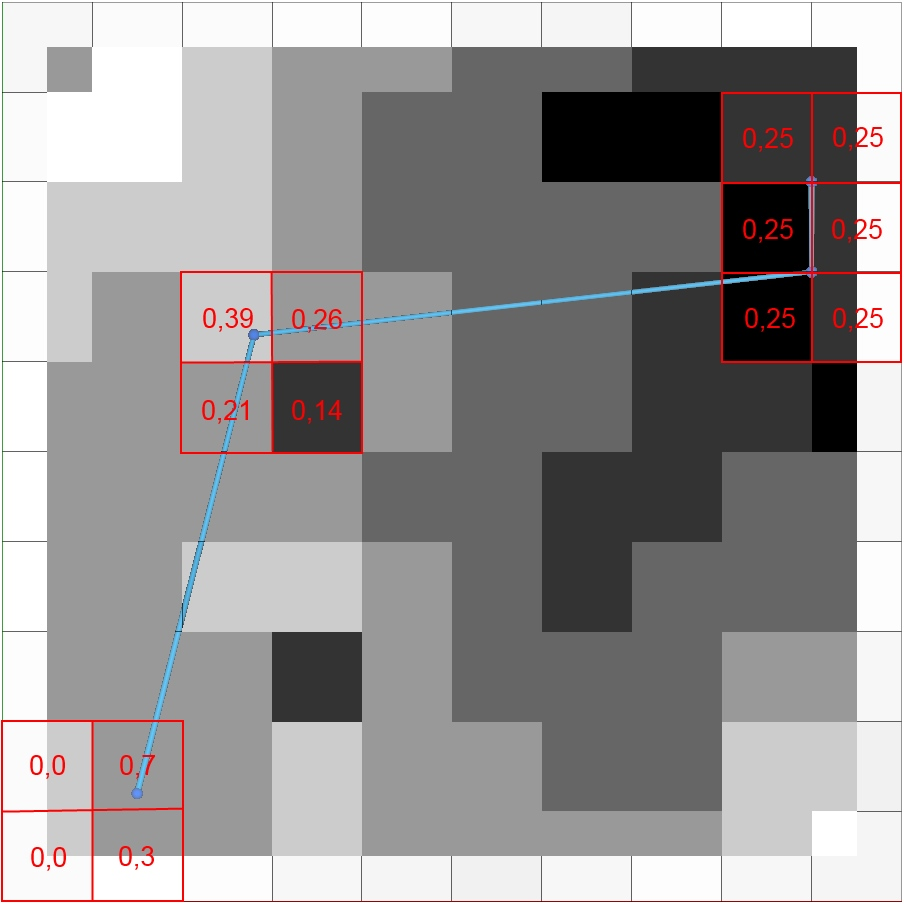
\includegraphics[width=.26\linewidth]{schema-dem}}\label{fig:schema:dem}}\,
  \subfloat[Mapping based on mesh]{\frame{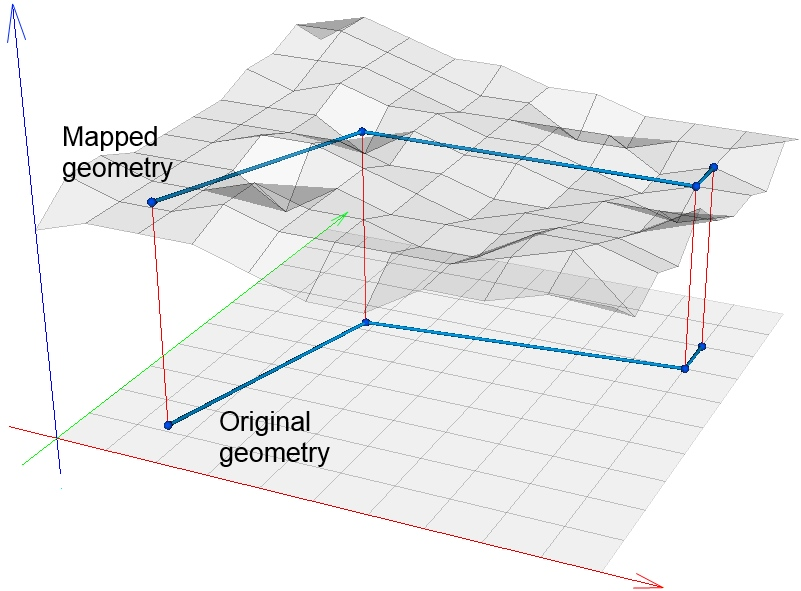
\includegraphics[width=.3525\linewidth]{schema-mesh1}}\label{fig:schema:mesh}}\,
  \subfloat[Additional geometric points]{\frame{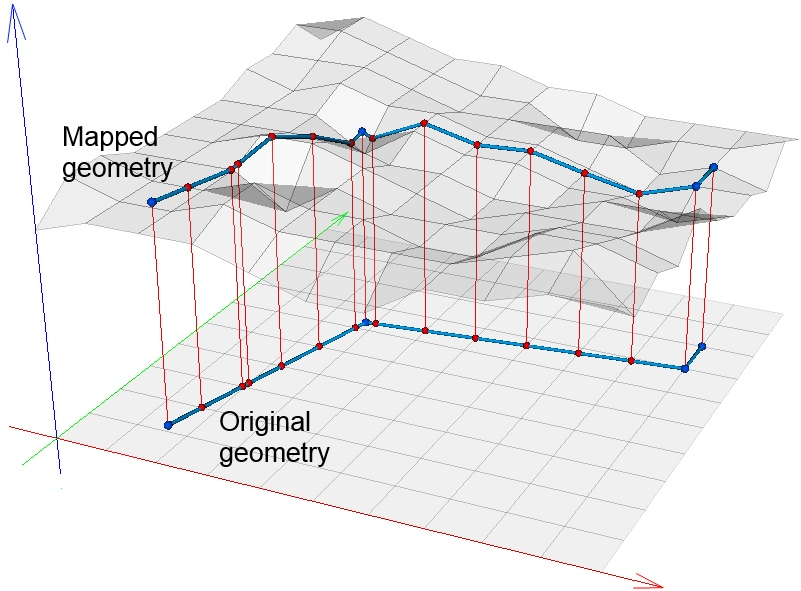
\includegraphics[width=.3525\linewidth]{schema-mesh2}}\label{fig:schema:points}}
  \caption{Schematic of mapping algorithms implemented in the \emph{OpenGeoSys Data Explorer}. \textbf{(a)}~Calculation of geometric point elevation based on weighted DEM pixels. \textbf{(b)}~Projection of points onto mesh surfaces via triangle line intersection. \textbf{(c)}~Inserting additional points into geometry at intersections of geometric lines with mesh element edges and nodes. Newly inserted points are marked in red.}
  \label{fig:geomappingschema}
\end{figure}

\subsection{Mapping Geometry}
\index{Mapping geometry}

Right-clicking a geometry in the Data View and selecting \cmd{Map geometry...} allows to add elevation information to all points of the selected geometry based on another data set (see fig. \ref{fig:dlgmods}a). This ``source''-data set can be either a mesh file or a file containing a digital elevation model (usually a *.asc or *.grd file). Both options can be selected from the pull down menu ``Map on data set''. In addition, this menu allows to select any mesh already loaded into \ogs to avoid loading the data set a second time. When selecting a DEM, geometric point will be given the elevation of the pixel they fall on when projected into the $(x,y)$-plane (see fig. \ref{fig:schema:dem}).

For a subsequent FEM-based simulation, it is usually better to map a geometric data set on the FEM mesh if the geometry will later be used for assigning boundary conditions. The mapping-dialogue offers two options for this case:

\begin{enumerate}
\item All geometric points $p_i \in P$ are mapped to the exact elevation of the mesh at the position of the point $p_i$ in the $(x,y)$-plane, i.e. to the point where a vertical line through $p_i$ intersects the mesh (see fig. \ref{fig:schema:mesh}).
\item In addition to the previous method, additional points are added whenever polylines projected onto the $(x,y)$-plane intersect mesh nodes or edges that have also been projected onto the $(x,y)$-plane (see \ref{fig:schema:points}).
\end{enumerate}

The second method will often result in larger geometry data sets, but also in a much better mapping. If unsure which method to use, it makes sense to try both and select the subjectively best result afterwards.


\section{Time Series and Stratigraphic Data to Observation Sites}
\index{Time series data}\index{Stratigraphic data}

For observation sites within the ``Stations'' Data View it is possible to display additional information such as logger data at the site or the stratigraphy at a borehole.

To view the additional information of an observation site load a stn-file into the programme and right-click on any observation site in the data view. You will see either the menu entry ``View Stratigraphy...'' for a borehole or ``View Diagram...'' for a station. While a borehole will always have strategraphic data (at least one layer over its whole length), not all stations will have time series data attached (this needs to be specified in the input file). If such data exists, a dialogue will open which allows to set a few parameters: A start and end date are set based on the data in the attached time series file for this station. This date can be changed to only display a subset of the data. There are also checkboxes for all all time series contained in the file which allow to specifically select only the time series the user wants to see. Upon pressing OK a new window will open, displaying the requested information.

\section{Generating and Modifying Meshes}

This section summarises the various way meshes can be created or modified using OpenGeoSys. Often functionality will be limited to a certain type of meshes, i.e. 2D meshes or 3D meshes. Usually the mesh dimension is based on the dimension of the elements within that mesh. For example, a triangle-mesh is 2D, a tetrahedra-mesh is 3D. For mixed element meshes, we find the maximum dimension of all the elements contained in that mesh to determine the mesh dimension. For example, a mesh containing tetrahedra (3D) and triangles (2D) is a 3D mesh; a mesh containing quads (2D) and lines (1D) is a 2D mesh; etc.

\subsection{Creating Meshes from Geometry}
\label{meshcreation}\index{Creating meshes}

By selecting \cmd{Tools\ra Mesh Generation...} a dialogue that allows the user to create meshes using information currently present in the programme. For this to work, the open-source mesh generating software GMSH\footnote{http://geuz.org/gmsh/} needs to be installed and be available from the location of the Data Explorer (i.e. located in the same directory or findable, e.g. via PATH-variable under MS Windows).

The user can select any geometry and observation sites that should be considered for generating the mesh. It is necessary that at least on polyline in any of the selected geometries is closed (i.e. is a polygon) and will serve as an outer boundary to the resulting mesh. Any further polygons found in the geometry will be meshed, polygons within polygons will simply be integrated within the encompassing larger shape. Note that all points of every data set considered for mesh generation and located within the outer boundary will be included as nodes in the final mesh. Therefore it makes sense to check if consecutive points of polylines are unnecessarily close together or too far apart.

Upon pressing \cmd{OK} a geometry-file (*.geo) for GMSH is written, GMSH is called to create the mesh and the newly created mesh is at once imported in the \ogs-Data Explorer. If not specified otherwise, the geo-file will be deleted again after the mesh has been created.

There is an \cmd{Advanced}-Tab in this dialogue that allows to set a number of parameters for the mesh. Most importantly, it can be chosen, if the new mesh should be adaptive or homogeneous. An adaptive mesh{Adaptive Meshes} is refined towards points or lines specified in the geometry while a homogeneous mesh has elements of roughly the same size everywhere in the domain (see figure \ref{fig:meshing}).

\begin{figure}[tb]
\begin{center}
\subfloat[Geometry]{\includegraphics[width=0.3\linewidth]{meshing-geo}\label{meshing-geo}}\enspace
\subfloat[Homogeneous mesh]{\includegraphics[width=0.3\linewidth]{meshing-hmg}\label{meshing-hmg}}\enspace
\subfloat[Adaptive mesh]{\includegraphics[width=0.3\linewidth]{meshing-adp}\label{meshing-adp}}
\end{center}
\caption{Meshing using geometric data and observation sites.} \label{fig:meshing}
\end{figure}

The specific parameters for adaptive meshes are:
\index{Adaptive meshes}
\begin{itemize}
\item \textbf{Max. number of points in Quadtree leaf:} Generally speaking, the smaller this number the more refined the resulting mesh will be. \\
    To give a more detailed explanation, basic knowledge about \emph{quad tree} data structures \footnote{http://en.wikipedia.org/wiki/Quadtree} is necessary: A tree structure is constructed by a sequential subdivision of the domain based on the distribution of relevant points in space. The criterium if a segment compromising a leaf is further refined is dependent on the number of points located within that segment. The size of the parameter relates to the maximum allowed size of mesh elements and additional points (\emph{Steiner points}) will be added to the data set to ensure the a certain refinement is guaranteed anywhere within the domain. Therefore, larger numbers of that parameters will usually result in coarser meshes while smaller numbers will result in finer meshes. \emph{Note that this is technically not a correct explanation as results are heavily dependent on how many points are located in certain sub-divisions of the domain, the existence of point clusters, etc.} See figure \ref{fig:quadtree} for an example.
\item \textbf{Mesh density scaling for points:} This is a scaling factor for the above parameter allowing for a refinement towards points located within the outer boundary. Again, smaller values will result in finer meshes.
\item \textbf{Mesh density scaling for stations:} This is exactly the same kind of scaling factor as for the option above, only for refinement towards observation sites, allowing a different mesh density for different regions of the mesh.
\end{itemize}

\begin{figure}[tb]
\begin{center}
\includegraphics[width=0.95\linewidth]{quadtree}\label{quadtree}
\end{center}
\caption{Adaptive meshing of geometry. The left column depicts polyline and points that need to be meshed. In the middle the resulting quad trees can be seen, the upper on generated with a maximum of two points per leaf, the lower one with 10 points per leaf. The resulting meshes are shown on the right side. Notice that regions where no information is available have roughly the same element size while elements where point information is given differ vastly in element size.} \label{fig:quadtree}
\end{figure}

Likewise, you can select an \textbf{element size}\index{Element size} for homogeneous meshes.\index{Homogeneous meshes} Here, too, a smaller number will result in a finer mesh, as the value specifies the maximum edge length of mesh elements.

\bigskip

Default parameters for all options are already predefined and have worked well with most examples that have been tested. However, results are heavily dependent an the bounding box of all data sets used for mesh generation. Often it is necessary to play around with these numbers a bit. Usually it makes sense to start with larger parameters that result in coarser meshes to get a rough idea what the final mesh will look like and where potential problems may be located.

\subsection{Creating Meshes from Raster Files}
\label{meshraster}\index{Creating meshes}

\begin{figure}[tb]
\begin{center}
\subfloat[Raster]{\includegraphics[width=0.3\linewidth]{rastermesh1}\label{rastermesh1}}\enspace
\subfloat[Elevation]{\includegraphics[width=0.3\linewidth]{rastermesh2}\label{rastermesh2}}\enspace
\subfloat[Materials]{\includegraphics[width=0.3\linewidth]{rastermesh3}\label{rastermesh3}}
\end{center}
\caption{Creating meshes from raster files: Pixels can be either represented as a set of two triangles (Fig. \ref{rastermesh2}) or a square (Fig. \ref{rastermesh3}), intensities may represent elevation (Fig. \ref{rastermesh2}) or materials (Fig. \ref{rastermesh3}).}
\label{fig:rastermesh}
\end{figure}

A completely different way to create a mesh is based on image or raster files, such as *.asc-files from ArcGIS. If the file is loading into the Data Explorer it will appear in the Visualisation Pipeline only. Right clicking the pipeline item allows to select the menu item \cmd{Convert Image to Mesh...}. A dialogue allows the parameterise how exactly this conversion should be performed. Specifically, it is possible to select a mesh element type for representation of pixels and a way in which grey-values should be interpreted\footnote{Meshes can also be generated from colour images. However, the colours will be converted to grey-values via $g = 0.3*\text{red}+0.6*\text{green}+0.1*\text{blue}$.}.

For the first parameter, pixels can be converted into a square (i.e. a quadrilateral element) or two rectilinear triangles (i.e. two triangle elements). In the future it is also planned to offer cubes (i.e. a hexahedron) for multi-layered images.

For the second parameter the user can decide wether pixel values should be interpreted as elevation (which is useful if the raster represents a digital elevation model) or if the grey-values should be assigned as scalar values to the mesh elements. As a third alternative, these values can also be completely ignored (see Fig. \ref{fig:rastermesh} for examples).

If the raster file contains ``NoData''-values (this is common in raster files created with a Geographic Information Systems such as ArcGIS), these values are ignored and will not appear as mesh-elements after the conversion  (i.e. despite the raster file always being rectilinear the resulting mesh may have an arbitrary boundary defined be pixels actually containing information).

\subsection{Converting Meshes to Geometry}
\index{Convert Mesh to geometry}
\index{Mesh to geometry conversion}

A 2D mesh loaded into \ogs can be converted into a geometry data set by right-clicking the mesh and selecting \cmd{Convert to geometry}. This will copy mesh nodes to geometric points and the mesh itself to a triangulated surface. In the same way, a 2D mesh can be converted into an ESRI shape file (by selecting \cmd{Export to Shapefile...}). The resulting file will be of type SHPT\textunderscore POLYGON and each mesh element will be represented as a polygon within the shape file.

\subsection{Extracting the surface of a mesh}

It is possible to extract the surface of a 3D mesh by right-clicking the mesh and selecting \cmd{Extract surface}. This will result in a 2D mesh of the surface elements of the 3D mesh, i.e. all elements visible when viewing the mesh from $z+$ direction.

Topologically, the result will consisting of all faces of 3D mesh elements where the surface normal n satisfies $|n - \left[0, 0, 1\right]|<90\degree$. Note that for certain meshes the result might also contain elements not actually connected to the surface if these unconnected elements also satisfy the constraint given above (e.g. if the 3D mesh contained holes).


\subsection{Mapping of Meshes based on DEMs}
\index{Mapping meshes}
\index{Adding mesh layers based on DEM}

For mapping a 2D mesh based on a DEM or for adding multiple layers based on elevation profiles, right-click the mesh and select \cmd{Edit mesh...}. The dialogue will require the number of layers to be mapped for this mesh. A ``layer'' in the sense of the underlying simulation algorithms, consists of 3D elements. Therefore a 2D mesh technically consists of $0$ layers. Subsequently, when mapping a 2D mesh, it is necessary to specify the number of layers as $0$ and use one DEM to actually map the layer. Likewise, one layer will require (at least) two digital elevation models (DEM) to be specified, one for the top-face of the elements and one for the bottom-face.

In general, $n+1$ raster files in *.asc format are required for mapping $n$ mesh layers. The dialogue also allows to select one additional DEM-file called ``Surface''. If a 2D mesh should be mapped, this is the only file that needs to be specified. For a 3D mesh it is optional and serves a different purpose: The raster files given for the mapping usually represent the boundaries between subsurface layers (e.g. Statigraphic layers, aquifers, etc.). These are often interpolated from borehole information (e.g. using the kriging algorithm). This may result in an upper boundary of the subsurface model that is located above the actual surface of the model region. For multi-layered meshes the mapping will first be performed on all subsurface layers and the resulting mesh will then be intersected with the optional Surface DEM (i.e. the digital terrain model), thus effectively cutting away all elements located above surface. \emph{Note that currently the check if two layers are intersecting each other does \emph{not} work correctly for any other layers except the DEM!}

\begin{figure}[tb]
\begin{center}
\subfloat[Surface Mesh]{\includegraphics[width=0.3\linewidth]{AmmerSurface}\label{fig:AmmerSurface}}\enspace
\subfloat[Fixed thickness]{\includegraphics[width=0.3\linewidth]{AmmerSubsurface}\label{fig:AmmerSubsurface}}\enspace
\subfloat[Based on DEM]{\includegraphics[width=0.3\linewidth]{AmmerFinal}\label{fig:AmmerFinal}}
\end{center}
\caption{Mapping meshes based on raster files: \textbf{(a)} original surface mesh, \textbf{(b)} adding subsurface layers of fixed size, \textbf{(c)} adding subsurface layers based on elevation models. In a final step the subsurface model is intersected with the terrain model (i.e. the actual surface elevation).}
\label{fig:RasterMapping}
\end{figure}

For meshes containing only 2D elements there is also an option ``Remove mesh nodes at NoData values''. Per default this option is switched off as the correctness of the result is depending on the element size in these NoData locations.

\subsection{Adding Layers of Fixed Size}
\index{Adding mesh layers of fixed size}

Besides adding subsurface layers using DEM-profiles as described in the previous section, a 2D mesh can also be extruded into a 3D mesh by copying the 2D mesh layer a specified number of times and then connected any two neighbouring layers by creating 3D elements from all corresponding 2D elements (i.e. two triangles are connected and form one prism-elements, two quadrilateral elements form one hexahedron). This functionality can also be accessed by right-clicking on a 2D mesh in the data view and selecting \cmd{Edit Mesh...}. Again, specify the number of layers you would like to add and select \cmd{Add layers with static thickness}. After that the thickness of each layer needs to be specified.

\subsection{Analyse Mesh Quality}
\index{Mesh quality}

You can visualise the quality of a given mesh by right-clicking on the mesh in the respective Data View and selecting \cmd{Check Mesh Quality...}. This currently allows to choose between four implemented measurements for mesh element quality. The result of choosing any of these modes is a colour-codes overlay of the mesh where every element is assigned a quality in $[0,1]$. You can select this overlay in the visualisation pipeline and specify thresholds to select a certain range of quality and see which element fall into that range. \emph{(Note: You might need to manually set the correct scalar array for visualising mesh quality. The appropriate data can be chosen by selecting in ``C-Selection'' in the \cmd{Active Scalar} pull-down menu.}

\begin{figure}[tb]
\begin{center}
\subfloat[Edge Aspect Ratio]{\includegraphics[width=0.3\linewidth]{MshQualEdgeRatio}\label{fig:mshqual1}}\enspace
\subfloat[Element Area]{\includegraphics[width=0.3\linewidth]{MshQualArea}\label{fig:mshqual2}}\enspace
\subfloat[EquiAngle Skewness]{\includegraphics[width=0.3\linewidth]{MshQualEquiAngle}\label{fig:mshqual3}}
\end{center}
\caption{Examples for colour coded mesh quality measurements.} \label{fig:mshqual}
\end{figure}

The currently implemented measures are the following:
\begin{itemize}
\item \textbf{Aspect Ratio of Edge Length:} Analyses the ratio of shortest to longest edge of every element. Equilateral elements are often considered superior and better suited for FEM simulation, therefore these elements are rated ``1'' with their quality degrading with increasing differences in edge length. Each element is assigned the value of the highest ratio between any two of its edges. This is a good measure for triangle elements but might be not as good as others. See figure \ref{fig:mshqual1}.
\item \textbf{Area of 2D Elements:} Compares the area of all 2D elements (this includes the faces of 3D elements!) by assigned ``1'' to the element with the largest area and ``0'' to the element with the smallest area. See figure \ref{fig:mshqual2}.
\item \textbf{Volume of 3D Elements:} As with the area-criterion, this measure compares the volume of 3D mesh elements. 2D elements are ignored when this option is selected.
\item \textbf{Angles between Adjacent Edges:} Calculates the maximum deviation of an angle between any two adjacent edges of the element from the ``optimum'' angle, i.e. the angle of an equiangular element. This optimum angle is $90\degree$ for triangles or tetrahedra and $90\degree$ for quadrilateral or hexahedral elements. This measurement is called \emph{EquiAngle Skewness} and given by
    \begin{equation}
    s = \max\left[\frac{\theta_{max}-\theta_{opt}}{180-\theta_{opt}},\frac{\theta_{opt}-\theta_{min}}{\theta_{opt}}\right]
    \end{equation}
    where $\theta_{max}$ is the maximum angle between any two edges found in the element, $\theta_{min}$ is the minimum angle and $\theta_{opt}$ is the optimum angle.
    See figure \ref{fig:mshqual3}.
\end{itemize}

The quality measure best suited for a given mesh might depend on the process you want to simulate using this mesh. For instance, processes such as groundwater recharge consist mainly of layered flows, meaning that large differences between horizontal and vertical element surfaces might have no effect on a correct result. The simulation of mass transport processes explicitly requires a fine mesh resolution in vertical direction to ensure a stable solution.

\begin{figure}[tb]
\begin{center}
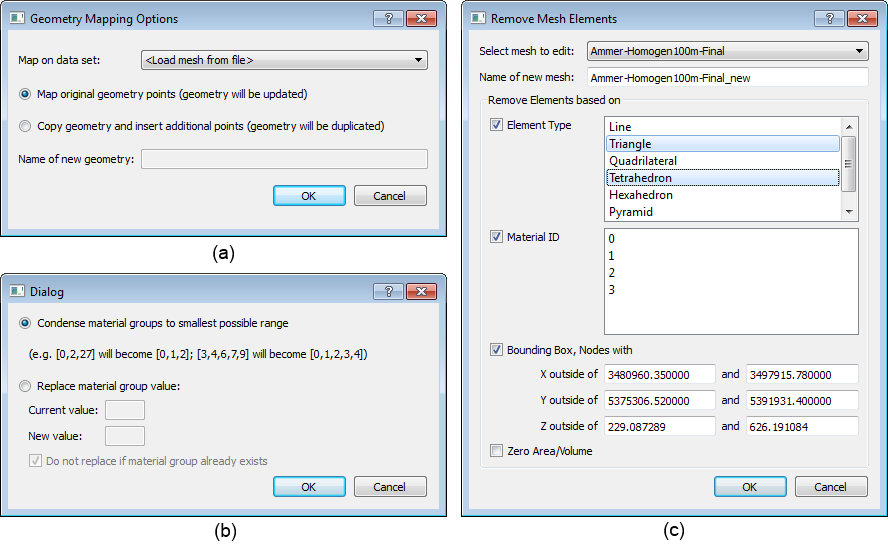
\includegraphics[width=0.8\linewidth]{dlg_mods}
\end{center}
\caption{\ogs Data Explorer dialogs for modification of data sets: \textbf{(a)} Mapping geometry based on a mesh or DEM, \textbf{(b)} Changing the material groups of a mesh, \textbf{(c)} Remove elements from a mesh based on certain criteria.} \label{fig:dlgmods}
\end{figure}

\subsection{Changing Material Groups}
\index{Changing material groups}

Each element in a mesh is assigned a non-negative integer that specifies a material group this element belongs to. These material groups can be arbitrarily assigned. For instance, a mesh containing only two groups could name these groups ``17'' and ``98'' or use some different, arbitrary IDs. By right-clicking on a mesh and selecting \cmd{Edit Material Groups...} it is possible the change the ID of one or more groups or to merge groups (see fig. \ref{fig:dlgmods}b).

The two basic options are ``Condense material groups to smallest possible range'' and ``Replace material group value''. The first option will rename all material groups such that the group with the smallest ID will be assigned $0$, the group with the second-smallest ID will be assigned $1$, and so on. In a mesh with $10$ different material groups the largest existing ID will be $9$ after processing the mesh.

The second option allows to specifically rename the ID of any group from the current value $A$ to any new value $B$. If $B$ already exists, the programme will give a warning and ask the user if the renaming process should really be started, thus merging groups $A$ and $B$.

\subsection{Removing Duplicate or Unused Mesh Nodes}
\index{Removing mesh nodes}

As with loading geometric data, certain checks are performed when loading meshes. The programme will automatically removed mesh nodes that are not part of any mesh element. Also, it is possible to remove duplicate mesh nodes, i.e. nodes that are located at the exact or almost exact same position as other nodes. The results for meshes are a bit more complicated as for geometries and this might require a restructuring or subdivision of mesh elements (i.e. if one node is removed from a prism-element, restructuring will result in two tetrahedra).

\subsection{Removing Mesh Elements}
\index{Removing mesh elements}

\ogs allows to remove mesh elements based on a number of criteria. A dialogue for selecting which elements to remove can by opened by selecting \cmd{Tools \ra Remove Mesh Elements...} (see fig. \ref{fig:dlgmods}c). It is necessary to specify the mesh from which elements need to be removed as well as the name of the resulting new mesh. Possible options based on which elements may be removed include element type, material group, bounding box as well as zero volume elements. The dialogue allows to select any combination of these constraints. An error message will be given if the selected criteria would result in removing either none or all of the elements in the selected mesh.



\section{Modelling Data}

\subsection{Creating Processes}
\index{Creating processes}

It is possible to add processes to the workflow in the Modelling-tab by pressing the \cmd{Add process...}-button. A dialogue will open that allows to select a process type and an associated primary variable. As of version 5.2.07 this has no effect on output files except for boundary conditions being grouped under these processes and being removed upon removing the process (via right-click \cmd{Remove process}).

\subsection{Creating FEM Conditions}
\index{Creating FEM conditions}
\index{Creating boundary conditions}

It is possible to create FEM conditions based on geometric objects. By right-clicking on the respective point, polyline or surface and selecting \cmd{Set as FEM condition...} a setup dialogue will open (Fig. \ref{fig:CondSetupDlg}). Here, it can be specified for which process and primary variable the condition should be used and if it should be a boundary condition, a source term or an initial condition. Based on the geometrical object type and the selection of the condition type a number of distribution types will be available. For example, points as boundary conditions can only have \emph{Constant (Dirichlet)} distribution; lines as source terms can have \emph{Constant (Neumann)} or \emph{Linear (Neumann)} distribution, etc.

\begin{figure}[tb]
\begin{center}
\subfloat[FEM Condition Setup]{\includegraphics[height=4.0cm]{dlg_cond_setup}\label{fig:CondSetupDlg}}\enspace
\subfloat[Linear]{\includegraphics[height=4.0cm]{dlg_lin_dist}\label{fig:LinearDlg}}\enspace
\subfloat[Direct]{\includegraphics[height=4.0cm]{dlg_direct_dist}\label{fig:DirectDlg}}
\end{center}
\caption{Dialogues for creating of FEM Conditions.} \label{fig:CondSetup}
\end{figure}

While the assignment of values is easy for \emph{constant} distributions, it an get quite complex for \emph{linear} or \emph{direct} distributions. The FEM Condition Setup Dialogue will therefore contain a button ``Calculate Values'' instead of a textfield. Upon pressing this button a (different) dialogue will open to configure the values. For \emph{linear} distributions a table is displayed where for each point of the line a value can be inserted (Fig. \ref{fig:LinearDlg}). Conditions are only actually set up between points with given values. As an alternative it is possible to automatically insert the elevation (z-Coordinate) for each point of the line. For \emph{direct} distributions the dialogue will require to specify a raster file from which values are read for direct assignment to mesh nodes (Fig. \ref{fig:DirectDlg}). The user can select between a 1:1 assignment or a surface integration based on the area of the mesh elements the respective node is part of. In this case it is also possible to specify a scaling value to compensate for data files with different units of measurement.

For polylines or surfaces it is also possible to assign the conditions not directly on the geometric objects but instead on all points compromising the object. For example, a polyline consisting of 50 points can be either assigned one boundary conditions with a linear distribution or 50 boundary conditions on the respective points, each of which has a constant value.

Once created, FEM conditions can be saved by right-clicking associated process in the ``Modelling'' tab and selecting \cmd{Save FEM conditions...}. The user can specify the file format (XML or ASCII) and the type of conditions that should be written (boundary conditions, initial conditions, source terms or all of them).

\subsection{Changing FEM Conditions}
\index{Changing FEM conditions}

Conditions loaded into the \ogs Data Explorer can be edited simply by right-clicking the respective geometric object in the ``Modelling'' tab and selecting \cmd{Edit condition}. This will once again open the FEM Condition Setup Dialogue that is also used for creating conditions. For existing conditions the appropriate values will already have been selected and can now be changed. Changes in the corresponding files will only be written once the user actively saves these files again via \cmd{Save FEM Conditions...}

